\documentclass{article}

% ============================================================
% INFR11269 Machine Learning Systems — Coursework Report
% Format rules (from the supplied template): do not edit the style file, page
% geometry, font size or line spacing; keep \iclrfinalcopy and the abstract
% commented out; main body at most six pages.
% ============================================================

\usepackage{iclr2027_conference,times}

\usepackage{hyperref}
\usepackage{url}
\usepackage{booktabs}
\usepackage{graphicx}
\usepackage{amsmath}
\usepackage{amssymb}

%%%%% NEW MATH DEFINITIONS %%%%%

\usepackage{amsmath,amsfonts,bm}

% Mark sections of captions for referring to divisions of figures
\newcommand{\figleft}{{\em (Left)}}
\newcommand{\figcenter}{{\em (Center)}}
\newcommand{\figright}{{\em (Right)}}
\newcommand{\figtop}{{\em (Top)}}
\newcommand{\figbottom}{{\em (Bottom)}}
\newcommand{\captiona}{{\em (a)}}
\newcommand{\captionb}{{\em (b)}}
\newcommand{\captionc}{{\em (c)}}
\newcommand{\captiond}{{\em (d)}}

% Highlight a newly defined term
\newcommand{\newterm}[1]{{\bf #1}}


% Figure reference, lower-case.
\def\figref#1{figure~\ref{#1}}
% Figure reference, capital. For start of sentence
\def\Figref#1{Figure~\ref{#1}}
\def\twofigref#1#2{figures \ref{#1} and \ref{#2}}
\def\quadfigref#1#2#3#4{figures \ref{#1}, \ref{#2}, \ref{#3} and \ref{#4}}
% Section reference, lower-case.
\def\secref#1{section~\ref{#1}}
% Section reference, capital.
\def\Secref#1{Section~\ref{#1}}
% Reference to two sections.
\def\twosecrefs#1#2{sections \ref{#1} and \ref{#2}}
% Reference to three sections.
\def\secrefs#1#2#3{sections \ref{#1}, \ref{#2} and \ref{#3}}
% Reference to an equation, lower-case.
\def\eqref#1{equation~\ref{#1}}
% Reference to an equation, upper case
\def\Eqref#1{Equation~\ref{#1}}
% A raw reference to an equation---avoid using if possible
\def\plaineqref#1{\ref{#1}}
% Reference to a chapter, lower-case.
\def\chapref#1{chapter~\ref{#1}}
% Reference to an equation, upper case.
\def\Chapref#1{Chapter~\ref{#1}}
% Reference to a range of chapters
\def\rangechapref#1#2{chapters\ref{#1}--\ref{#2}}
% Reference to an algorithm, lower-case.
\def\algref#1{algorithm~\ref{#1}}
% Reference to an algorithm, upper case.
\def\Algref#1{Algorithm~\ref{#1}}
\def\twoalgref#1#2{algorithms \ref{#1} and \ref{#2}}
\def\Twoalgref#1#2{Algorithms \ref{#1} and \ref{#2}}
% Reference to a part, lower case
\def\partref#1{part~\ref{#1}}
% Reference to a part, upper case
\def\Partref#1{Part~\ref{#1}}
\def\twopartref#1#2{parts \ref{#1} and \ref{#2}}

\def\ceil#1{\lceil #1 \rceil}
\def\floor#1{\lfloor #1 \rfloor}
\def\1{\bm{1}}
\newcommand{\train}{\mathcal{D}}
\newcommand{\valid}{\mathcal{D_{\mathrm{valid}}}}
\newcommand{\test}{\mathcal{D_{\mathrm{test}}}}

\def\eps{{\epsilon}}


% Random variables
\def\reta{{\textnormal{$\eta$}}}
\def\ra{{\textnormal{a}}}
\def\rb{{\textnormal{b}}}
\def\rc{{\textnormal{c}}}
\def\rd{{\textnormal{d}}}
\def\re{{\textnormal{e}}}
\def\rf{{\textnormal{f}}}
\def\rg{{\textnormal{g}}}
\def\rh{{\textnormal{h}}}
\def\ri{{\textnormal{i}}}
\def\rj{{\textnormal{j}}}
\def\rk{{\textnormal{k}}}
\def\rl{{\textnormal{l}}}
% rm is already a command, just don't name any random variables m
\def\rn{{\textnormal{n}}}
\def\ro{{\textnormal{o}}}
\def\rp{{\textnormal{p}}}
\def\rq{{\textnormal{q}}}
\def\rr{{\textnormal{r}}}
\def\rs{{\textnormal{s}}}
\def\rt{{\textnormal{t}}}
\def\ru{{\textnormal{u}}}
\def\rv{{\textnormal{v}}}
\def\rw{{\textnormal{w}}}
\def\rx{{\textnormal{x}}}
\def\ry{{\textnormal{y}}}
\def\rz{{\textnormal{z}}}

% Random vectors
\def\rvepsilon{{\mathbf{\epsilon}}}
\def\rvtheta{{\mathbf{\theta}}}
\def\rva{{\mathbf{a}}}
\def\rvb{{\mathbf{b}}}
\def\rvc{{\mathbf{c}}}
\def\rvd{{\mathbf{d}}}
\def\rve{{\mathbf{e}}}
\def\rvf{{\mathbf{f}}}
\def\rvg{{\mathbf{g}}}
\def\rvh{{\mathbf{h}}}
\def\rvu{{\mathbf{i}}}
\def\rvj{{\mathbf{j}}}
\def\rvk{{\mathbf{k}}}
\def\rvl{{\mathbf{l}}}
\def\rvm{{\mathbf{m}}}
\def\rvn{{\mathbf{n}}}
\def\rvo{{\mathbf{o}}}
\def\rvp{{\mathbf{p}}}
\def\rvq{{\mathbf{q}}}
\def\rvr{{\mathbf{r}}}
\def\rvs{{\mathbf{s}}}
\def\rvt{{\mathbf{t}}}
\def\rvu{{\mathbf{u}}}
\def\rvv{{\mathbf{v}}}
\def\rvw{{\mathbf{w}}}
\def\rvx{{\mathbf{x}}}
\def\rvy{{\mathbf{y}}}
\def\rvz{{\mathbf{z}}}

% Elements of random vectors
\def\erva{{\textnormal{a}}}
\def\ervb{{\textnormal{b}}}
\def\ervc{{\textnormal{c}}}
\def\ervd{{\textnormal{d}}}
\def\erve{{\textnormal{e}}}
\def\ervf{{\textnormal{f}}}
\def\ervg{{\textnormal{g}}}
\def\ervh{{\textnormal{h}}}
\def\ervi{{\textnormal{i}}}
\def\ervj{{\textnormal{j}}}
\def\ervk{{\textnormal{k}}}
\def\ervl{{\textnormal{l}}}
\def\ervm{{\textnormal{m}}}
\def\ervn{{\textnormal{n}}}
\def\ervo{{\textnormal{o}}}
\def\ervp{{\textnormal{p}}}
\def\ervq{{\textnormal{q}}}
\def\ervr{{\textnormal{r}}}
\def\ervs{{\textnormal{s}}}
\def\ervt{{\textnormal{t}}}
\def\ervu{{\textnormal{u}}}
\def\ervv{{\textnormal{v}}}
\def\ervw{{\textnormal{w}}}
\def\ervx{{\textnormal{x}}}
\def\ervy{{\textnormal{y}}}
\def\ervz{{\textnormal{z}}}

% Random matrices
\def\rmA{{\mathbf{A}}}
\def\rmB{{\mathbf{B}}}
\def\rmC{{\mathbf{C}}}
\def\rmD{{\mathbf{D}}}
\def\rmE{{\mathbf{E}}}
\def\rmF{{\mathbf{F}}}
\def\rmG{{\mathbf{G}}}
\def\rmH{{\mathbf{H}}}
\def\rmI{{\mathbf{I}}}
\def\rmJ{{\mathbf{J}}}
\def\rmK{{\mathbf{K}}}
\def\rmL{{\mathbf{L}}}
\def\rmM{{\mathbf{M}}}
\def\rmN{{\mathbf{N}}}
\def\rmO{{\mathbf{O}}}
\def\rmP{{\mathbf{P}}}
\def\rmQ{{\mathbf{Q}}}
\def\rmR{{\mathbf{R}}}
\def\rmS{{\mathbf{S}}}
\def\rmT{{\mathbf{T}}}
\def\rmU{{\mathbf{U}}}
\def\rmV{{\mathbf{V}}}
\def\rmW{{\mathbf{W}}}
\def\rmX{{\mathbf{X}}}
\def\rmY{{\mathbf{Y}}}
\def\rmZ{{\mathbf{Z}}}

% Elements of random matrices
\def\ermA{{\textnormal{A}}}
\def\ermB{{\textnormal{B}}}
\def\ermC{{\textnormal{C}}}
\def\ermD{{\textnormal{D}}}
\def\ermE{{\textnormal{E}}}
\def\ermF{{\textnormal{F}}}
\def\ermG{{\textnormal{G}}}
\def\ermH{{\textnormal{H}}}
\def\ermI{{\textnormal{I}}}
\def\ermJ{{\textnormal{J}}}
\def\ermK{{\textnormal{K}}}
\def\ermL{{\textnormal{L}}}
\def\ermM{{\textnormal{M}}}
\def\ermN{{\textnormal{N}}}
\def\ermO{{\textnormal{O}}}
\def\ermP{{\textnormal{P}}}
\def\ermQ{{\textnormal{Q}}}
\def\ermR{{\textnormal{R}}}
\def\ermS{{\textnormal{S}}}
\def\ermT{{\textnormal{T}}}
\def\ermU{{\textnormal{U}}}
\def\ermV{{\textnormal{V}}}
\def\ermW{{\textnormal{W}}}
\def\ermX{{\textnormal{X}}}
\def\ermY{{\textnormal{Y}}}
\def\ermZ{{\textnormal{Z}}}

% Vectors
\def\vzero{{\bm{0}}}
\def\vone{{\bm{1}}}
\def\vmu{{\bm{\mu}}}
\def\vtheta{{\bm{\theta}}}
\def\va{{\bm{a}}}
\def\vb{{\bm{b}}}
\def\vc{{\bm{c}}}
\def\vd{{\bm{d}}}
\def\ve{{\bm{e}}}
\def\vf{{\bm{f}}}
\def\vg{{\bm{g}}}
\def\vh{{\bm{h}}}
\def\vi{{\bm{i}}}
\def\vj{{\bm{j}}}
\def\vk{{\bm{k}}}
\def\vl{{\bm{l}}}
\def\vm{{\bm{m}}}
\def\vn{{\bm{n}}}
\def\vo{{\bm{o}}}
\def\vp{{\bm{p}}}
\def\vq{{\bm{q}}}
\def\vr{{\bm{r}}}
\def\vs{{\bm{s}}}
\def\vt{{\bm{t}}}
\def\vu{{\bm{u}}}
\def\vv{{\bm{v}}}
\def\vw{{\bm{w}}}
\def\vx{{\bm{x}}}
\def\vy{{\bm{y}}}
\def\vz{{\bm{z}}}

% Elements of vectors
\def\evalpha{{\alpha}}
\def\evbeta{{\beta}}
\def\evepsilon{{\epsilon}}
\def\evlambda{{\lambda}}
\def\evomega{{\omega}}
\def\evmu{{\mu}}
\def\evpsi{{\psi}}
\def\evsigma{{\sigma}}
\def\evtheta{{\theta}}
\def\eva{{a}}
\def\evb{{b}}
\def\evc{{c}}
\def\evd{{d}}
\def\eve{{e}}
\def\evf{{f}}
\def\evg{{g}}
\def\evh{{h}}
\def\evi{{i}}
\def\evj{{j}}
\def\evk{{k}}
\def\evl{{l}}
\def\evm{{m}}
\def\evn{{n}}
\def\evo{{o}}
\def\evp{{p}}
\def\evq{{q}}
\def\evr{{r}}
\def\evs{{s}}
\def\evt{{t}}
\def\evu{{u}}
\def\evv{{v}}
\def\evw{{w}}
\def\evx{{x}}
\def\evy{{y}}
\def\evz{{z}}

% Matrix
\def\mA{{\bm{A}}}
\def\mB{{\bm{B}}}
\def\mC{{\bm{C}}}
\def\mD{{\bm{D}}}
\def\mE{{\bm{E}}}
\def\mF{{\bm{F}}}
\def\mG{{\bm{G}}}
\def\mH{{\bm{H}}}
\def\mI{{\bm{I}}}
\def\mJ{{\bm{J}}}
\def\mK{{\bm{K}}}
\def\mL{{\bm{L}}}
\def\mM{{\bm{M}}}
\def\mN{{\bm{N}}}
\def\mO{{\bm{O}}}
\def\mP{{\bm{P}}}
\def\mQ{{\bm{Q}}}
\def\mR{{\bm{R}}}
\def\mS{{\bm{S}}}
\def\mT{{\bm{T}}}
\def\mU{{\bm{U}}}
\def\mV{{\bm{V}}}
\def\mW{{\bm{W}}}
\def\mX{{\bm{X}}}
\def\mY{{\bm{Y}}}
\def\mZ{{\bm{Z}}}
\def\mBeta{{\bm{\beta}}}
\def\mPhi{{\bm{\Phi}}}
\def\mLambda{{\bm{\Lambda}}}
\def\mSigma{{\bm{\Sigma}}}

% Tensor
\DeclareMathAlphabet{\mathsfit}{\encodingdefault}{\sfdefault}{m}{sl}
\SetMathAlphabet{\mathsfit}{bold}{\encodingdefault}{\sfdefault}{bx}{n}
\newcommand{\tens}[1]{\bm{\mathsfit{#1}}}
\def\tA{{\tens{A}}}
\def\tB{{\tens{B}}}
\def\tC{{\tens{C}}}
\def\tD{{\tens{D}}}
\def\tE{{\tens{E}}}
\def\tF{{\tens{F}}}
\def\tG{{\tens{G}}}
\def\tH{{\tens{H}}}
\def\tI{{\tens{I}}}
\def\tJ{{\tens{J}}}
\def\tK{{\tens{K}}}
\def\tL{{\tens{L}}}
\def\tM{{\tens{M}}}
\def\tN{{\tens{N}}}
\def\tO{{\tens{O}}}
\def\tP{{\tens{P}}}
\def\tQ{{\tens{Q}}}
\def\tR{{\tens{R}}}
\def\tS{{\tens{S}}}
\def\tT{{\tens{T}}}
\def\tU{{\tens{U}}}
\def\tV{{\tens{V}}}
\def\tW{{\tens{W}}}
\def\tX{{\tens{X}}}
\def\tY{{\tens{Y}}}
\def\tZ{{\tens{Z}}}


% Graph
\def\gA{{\mathcal{A}}}
\def\gB{{\mathcal{B}}}
\def\gC{{\mathcal{C}}}
\def\gD{{\mathcal{D}}}
\def\gE{{\mathcal{E}}}
\def\gF{{\mathcal{F}}}
\def\gG{{\mathcal{G}}}
\def\gH{{\mathcal{H}}}
\def\gI{{\mathcal{I}}}
\def\gJ{{\mathcal{J}}}
\def\gK{{\mathcal{K}}}
\def\gL{{\mathcal{L}}}
\def\gM{{\mathcal{M}}}
\def\gN{{\mathcal{N}}}
\def\gO{{\mathcal{O}}}
\def\gP{{\mathcal{P}}}
\def\gQ{{\mathcal{Q}}}
\def\gR{{\mathcal{R}}}
\def\gS{{\mathcal{S}}}
\def\gT{{\mathcal{T}}}
\def\gU{{\mathcal{U}}}
\def\gV{{\mathcal{V}}}
\def\gW{{\mathcal{W}}}
\def\gX{{\mathcal{X}}}
\def\gY{{\mathcal{Y}}}
\def\gZ{{\mathcal{Z}}}

% Sets
\def\sA{{\mathbb{A}}}
\def\sB{{\mathbb{B}}}
\def\sC{{\mathbb{C}}}
\def\sD{{\mathbb{D}}}
% Don't use a set called E, because this would be the same as our symbol
% for expectation.
\def\sF{{\mathbb{F}}}
\def\sG{{\mathbb{G}}}
\def\sH{{\mathbb{H}}}
\def\sI{{\mathbb{I}}}
\def\sJ{{\mathbb{J}}}
\def\sK{{\mathbb{K}}}
\def\sL{{\mathbb{L}}}
\def\sM{{\mathbb{M}}}
\def\sN{{\mathbb{N}}}
\def\sO{{\mathbb{O}}}
\def\sP{{\mathbb{P}}}
\def\sQ{{\mathbb{Q}}}
\def\sR{{\mathbb{R}}}
\def\sS{{\mathbb{S}}}
\def\sT{{\mathbb{T}}}
\def\sU{{\mathbb{U}}}
\def\sV{{\mathbb{V}}}
\def\sW{{\mathbb{W}}}
\def\sX{{\mathbb{X}}}
\def\sY{{\mathbb{Y}}}
\def\sZ{{\mathbb{Z}}}

% Entries of a matrix
\def\emLambda{{\Lambda}}
\def\emA{{A}}
\def\emB{{B}}
\def\emC{{C}}
\def\emD{{D}}
\def\emE{{E}}
\def\emF{{F}}
\def\emG{{G}}
\def\emH{{H}}
\def\emI{{I}}
\def\emJ{{J}}
\def\emK{{K}}
\def\emL{{L}}
\def\emM{{M}}
\def\emN{{N}}
\def\emO{{O}}
\def\emP{{P}}
\def\emQ{{Q}}
\def\emR{{R}}
\def\emS{{S}}
\def\emT{{T}}
\def\emU{{U}}
\def\emV{{V}}
\def\emW{{W}}
\def\emX{{X}}
\def\emY{{Y}}
\def\emZ{{Z}}
\def\emSigma{{\Sigma}}

% entries of a tensor
% Same font as tensor, without \bm wrapper
\newcommand{\etens}[1]{\mathsfit{#1}}
\def\etLambda{{\etens{\Lambda}}}
\def\etA{{\etens{A}}}
\def\etB{{\etens{B}}}
\def\etC{{\etens{C}}}
\def\etD{{\etens{D}}}
\def\etE{{\etens{E}}}
\def\etF{{\etens{F}}}
\def\etG{{\etens{G}}}
\def\etH{{\etens{H}}}
\def\etI{{\etens{I}}}
\def\etJ{{\etens{J}}}
\def\etK{{\etens{K}}}
\def\etL{{\etens{L}}}
\def\etM{{\etens{M}}}
\def\etN{{\etens{N}}}
\def\etO{{\etens{O}}}
\def\etP{{\etens{P}}}
\def\etQ{{\etens{Q}}}
\def\etR{{\etens{R}}}
\def\etS{{\etens{S}}}
\def\etT{{\etens{T}}}
\def\etU{{\etens{U}}}
\def\etV{{\etens{V}}}
\def\etW{{\etens{W}}}
\def\etX{{\etens{X}}}
\def\etY{{\etens{Y}}}
\def\etZ{{\etens{Z}}}

% The true underlying data generating distribution
\newcommand{\pdata}{p_{\rm{data}}}
% The empirical distribution defined by the training set
\newcommand{\ptrain}{\hat{p}_{\rm{data}}}
\newcommand{\Ptrain}{\hat{P}_{\rm{data}}}
% The model distribution
\newcommand{\pmodel}{p_{\rm{model}}}
\newcommand{\Pmodel}{P_{\rm{model}}}
\newcommand{\ptildemodel}{\tilde{p}_{\rm{model}}}
% Stochastic autoencoder distributions
\newcommand{\pencode}{p_{\rm{encoder}}}
\newcommand{\pdecode}{p_{\rm{decoder}}}
\newcommand{\precons}{p_{\rm{reconstruct}}}

\newcommand{\laplace}{\mathrm{Laplace}} % Laplace distribution

\newcommand{\E}{\mathbb{E}}
\newcommand{\Ls}{\mathcal{L}}
\newcommand{\R}{\mathbb{R}}
\newcommand{\emp}{\tilde{p}}
\newcommand{\lr}{\alpha}
\newcommand{\reg}{\lambda}
\newcommand{\rect}{\mathrm{rectifier}}
\newcommand{\softmax}{\mathrm{softmax}}
\newcommand{\sigmoid}{\sigma}
\newcommand{\softplus}{\zeta}
\newcommand{\KL}{D_{\mathrm{KL}}}
\newcommand{\Var}{\mathrm{Var}}
\newcommand{\standarderror}{\mathrm{SE}}
\newcommand{\Cov}{\mathrm{Cov}}
% Wolfram Mathworld says $L^2$ is for function spaces and $\ell^2$ is for vectors
% But then they seem to use $L^2$ for vectors throughout the site, and so does
% wikipedia.
\newcommand{\normlzero}{L^0}
\newcommand{\normlone}{L^1}
\newcommand{\normltwo}{L^2}
\newcommand{\normlp}{L^p}
\newcommand{\normmax}{L^\infty}

\newcommand{\parents}{Pa} % See usage in notation.tex. Chosen to match Daphne's book.

\DeclareMathOperator*{\argmax}{arg\,max}
\DeclareMathOperator*{\argmin}{arg\,min}

\DeclareMathOperator{\sign}{sign}
\DeclareMathOperator{\Tr}{Tr}
\let\ab\allowbreak


\newcommand{\enca}{\texttt{enc\_a}}
\newcommand{\encb}{\texttt{enc\_b}}

\title{Serving a Half-Migrated Index: Encoder Migration in a Spoken-Question RAG System, and a 4.5$\times$ Faster ASR Front End}

% Keep this line unchanged.
\author{Anonymous coursework submission}

% Keep this COMMENTED OUT.
% \iclrfinalcopy

\begin{document}

\maketitle

% Course-specific template fingerprint. Keep this line unchanged.
\lhead{Under review as a report for UoE 26/27 Sem1 INFR11269: Machine Learning Systems}

% Keep this COMMENTED OUT.
% \begin{abstract}
% \end{abstract}

\section{Introduction}
\label{sec:introduction}

The course system answers spoken finance questions: a speech recogniser (GLM-ASR-Nano) transcribes the
audio, an encoder embeds the transcript, exact dense search returns the top records from a 24,000-record
corpus, and an LLM writes an answer from the top five \citep{lewis2020rag}. We ask three questions about it.

\textbf{Main question: how should a partly re-encoded index be searched?} Suppose the corpus was indexed with
a legacy encoder (\encb) and is being re-encoded with a new one (\enca) record by record, while queries keep
arriving. Only \enca\ can encode queries, so for a while the index holds two kinds of vectors. Re-encoding
everything before serving is the clean answer, but it means a second full index and a cut-over; serving
during the migration is what a live system has to do. We compare five ways to search the mixed index on
retrieval quality, answer quality and serving cost, at every stage of the migration.

\textbf{Extension: what does the ASR front end cost, and where does the time go?} We completed the four CUDA
kernel tasks (RoPE, reductions, tiled GEMM, attention) and then removed two sources of wasted work in the
supplied model: the 30-second padding of every clip, and the decoder's lack of a key/value cache.

\textbf{Secondary: where does the baseline's own retrieval fail, and can a later stage fix it?} We located
the baseline's failures and tested a cross-encoder reranker and an LLM query correction, each applied only to
queries the search is unsure about.

\textbf{Findings.} (1) Mixing two encoders' scores in one ranked list is the main failure: with 10\% of the
index migrated, Recall@10 falls from 0.475 to 0.205 (naive) or 0.079 (raw legacy vectors), because \enca\
records score higher \emph{as numbers}, not because they are more relevant. Mapping legacy vectors into the
\enca\ space with one least-squares fit (\emph{map-docs}) keeps 97--100\% of baseline quality at every fraction,
at no extra search cost, and its answers beat the naive strategy by +0.060 judge score (95\% CI
$[+0.006, +0.115]$). (2) Trimming the padding and adding a KV cache make transcription 4.5$\times$ faster on our
kernels; the KV cache changes no transcript and trimming changes 11 of 101, almost all in formatting. The
same KV cache gives nothing on PyTorch: whether an
optimisation pays depends on what the implementation is bound by. (3) Retrieval is the baseline's bottleneck,
but neither later stage pays for itself: reranking lowers NDCG@10 and costs 5\,s per query, and LLM query
correction gains +0.022 NDCG@10 (interval touching zero) for 2.5\,s per query.

\section{System and Technical Approach}
\label{sec:approach}

\textbf{Supplied system.} GLM-ASR-Nano computes a log-mel spectrogram, runs a 32-layer audio encoder over
1,500 frames (width 1,280), a projector and a 28-layer decoder (width 2,048, 16 query heads sharing 4
key/value heads \citep{ainslie2023gqa}) that decodes greedily in float32. The processor pads every clip to
30\,s, as in Whisper \citep{radford2023whisper}; a typical question is about 5\,s. The decoder has no KV cache:
each new token re-runs the whole sequence (prompt of 42--125 positions, median 76, plus the tokens so far). In the RAG pipeline \enca\ (384 dimensions)
embeds queries and records; \encb\ vectors (also 384-d) are supplied for the corpus only, without a query
encoder. Equal dimensions do not make the spaces compatible.

\textbf{CUDA kernels (our work).} RoPE \citep{su2021roformer} rotates one $(q,k)$ pair per thread, queries and
keys in one launch. Reductions use warp shuffles and one shared-memory slot per warp; softmax keeps a running
(max, sum) pair \citep{milakov2018online}, so it reads each element twice instead of three times. The GEMM
stages $16\times16$ tiles of $x$ and $W$ in shared memory (256 threads per block, one output each; every loaded
value is reused 16 times), pads each row of the $W$ tile by one float, so the 16 threads that read one column
hit 16 shared-memory banks instead of 2, and fuses bias and GELU into the store. Attention follows FlashAttention \citep{dao2022flashattention}: each warp owns
one query, keys and values stream through shared memory 32 at a time, and the score matrix is never stored.
Causal masking aligns the last query with the last key, so the same kernel serves the cached decoder below.

\textbf{ASR speed-ups (our work).} \emph{Trim}: the encoder receives only the frames the processor marks as
real, so a 5\,s clip gives about 250 encoder positions instead of 1,500. \emph{KV cache}: the prompt runs once,
then each step feeds only the new token and appends its keys and values to a per-layer cache
\citep{pope2023inference}. The supplied RoPE kernel numbers positions from 0 and its signature must not change;
for a token at position $p$ we rotate a two-row buffer with the frequencies scaled by $p$, so its second row
receives exactly the angle of position $p$. Both changes are switches in \texttt{model.py}; the five kernel files
are untouched by them.

\textbf{Migration strategies (our work).} At migrated fraction $f$, a random $f$ of the records have \enca\
vectors and the rest only \encb. Two $384\times384$ least-squares maps (A$\to$B and B$\to$A,
cf.\ \citealp{mikolov2013exploiting}) are fitted on records present in both spaces: 2,000 seed pairs plus every
migrated record. The query is always encoded with \enca.
\begin{itemize}
\item \textbf{no-map}: score legacy records with the raw \enca\ query against raw \encb\ vectors.
\item \textbf{naive}: migrated records with the \enca\ query; legacy records with the query mapped A$\to$B; one list.
\item \textbf{z-calibrated}: as naive, but each part's scores are standardised per query before merging.
\item \textbf{dual-read}: rank each part separately and merge with reciprocal rank fusion \citep{cormack2009rrf}.
\item \textbf{map-docs}: map legacy \emph{record} vectors B$\to$A once, then search one index with one query.
\end{itemize}
This is the serving-time view of backward-compatible representations \citep{shen2020bct}: rather than training
\enca\ to be compatible, we align the old vectors after the fact.

\textbf{Correcting the baseline's retrieval (our work).} A free confidence signal, the \emph{margin} (score of
result 1 minus score of result 10), selects the queries a costly stage is applied to, lowest margin first.
\emph{Reranking}: a MiniLM cross-encoder \citep{nogueira2019passage} re-scores the \enca\ top 50.
\emph{Correction}: one ELM call either rewrites the transcript as a clear finance question or writes a short
hypothetical answer (HyDE, \citealp{gao2023hyde}); we search with the corrected text alone, fuse its ranking
with the original, or sum the two query vectors (\emph{mix}). We also tried BM25 \citep{robertson2009bm25} and
\encb\ as extra first stages, and chunked records.

\section{Experimental Methodology}
\label{sec:methodology}

\textbf{Data and splits.} Retrieval uses the 125 dev questions (reported) and the 350 practice questions
(checked for the same pattern; Appendix~\ref{app:tables}), with the public relevance judgements. Query
transcripts come from the supplied ASR, cached once, so every strategy sees identical queries. The ASR
benchmark uses \texttt{test\_audio.wav} and the first 100 practice questions.

\textbf{Quality.} Retrieval: Recall@10 (main), NDCG@10, MRR@10 and Recall@100, mean and standard deviation
over five random migration orders. Answers: at 10\% migrated, the ELM (EuroLLM-22B) answers every dev
question from the top five records of each index state, and the course judge scores each answer once
(correctness, grounding, completeness; normalised to 0--1; supplied settings: answers at temperature 0.1,
judge at 0, the same EuroLLM-22B model for both). We compare states on the queries scored in all
of them (124 of 125) with paired bootstrap 95\% intervals \citep{efron1993bootstrap}. ASR: the transcript must be
identical to, or compared word by word with, the supplied model's; we also re-run retrieval on the new
transcripts. Correction settings were chosen on practice and are reported on dev; each is compared with
correcting the same number of randomly chosen queries.

\textbf{Cost.} Retrieval: search latency per query (one query at a time, CPU, mean of 200 repeated searches), index memory,
map fitting and mapping time. ASR: milliseconds per transcription and per generated token, encoder time, peak
GPU memory and GPU time per operation from \texttt{./run.sh --profile}.

\textbf{Controls.} All GPU numbers come from one NVIDIA GeForce RTX 2080 Ti (Teaching partition). In the ASR
benchmark the model is loaded once, every clip is transcribed with every variant in rotating order after a
warm-up, and medians over 101 clips are reported, so variants share GPU state and clock. Each comparison
changes one thing: the same seeds for all strategies, the same answer prompt and judge for all index states.

\section{Results and Analysis}
\label{sec:results}

\subsection{Migration: retrieval quality and cost}

\begin{figure}[t]
\centering
\begin{minipage}[t]{0.49\linewidth}
\centering
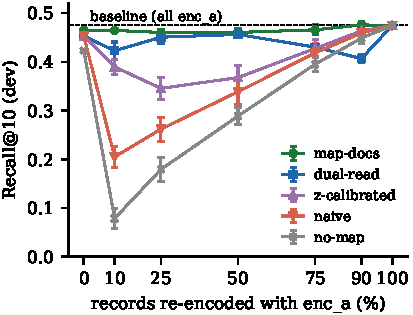
\includegraphics[width=\linewidth]{figures/migration_recall.pdf}
\caption{Recall@10 on dev against the share of records re-encoded with \enca\ (mean $\pm$ std over five
migration orders).}
\label{fig:migration}
\end{minipage}\hfill
\begin{minipage}[t]{0.49\linewidth}
\centering
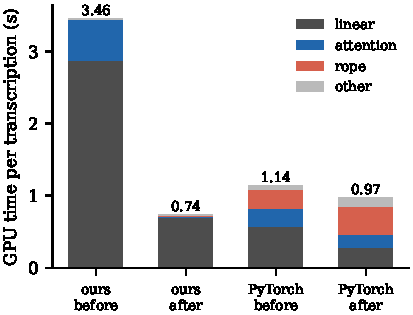
\includegraphics[width=\linewidth]{figures/asr_profile.pdf}
\caption{Profiled GPU time per operation for \texttt{test\_audio.wav}, before and after trim + KV cache.}
\label{fig:asr}
\end{minipage}
\end{figure}

\begin{table}[t]
\caption{Dev retrieval (125 questions) at three stages of the migration, and serving cost at 50\% (CPU, one
query at a time). Baseline (all \enca): Recall@10 0.475, NDCG@10 0.398.}
\label{tab:migration}
\centering
\small
\begin{tabular}{lcccccccc}
\toprule
& \multicolumn{3}{c}{Recall@10} & \multicolumn{3}{c}{NDCG@10} & \multicolumn{2}{c}{Cost at 50\%} \\
\cmidrule(lr){2-4}\cmidrule(lr){5-7}\cmidrule(lr){8-9}
Strategy & 10\% & 50\% & 90\% & 10\% & 50\% & 90\% & ms/query & index MB \\
\midrule
no-map       & 0.079 & 0.289 & 0.449 & 0.080 & 0.248 & 0.373 & 0.27 & 36.9 \\
naive        & 0.205 & 0.339 & 0.459 & 0.181 & 0.288 & 0.379 & 0.30 & 37.5 \\
z-calibrated & 0.390 & 0.368 & 0.463 & 0.289 & 0.303 & 0.381 & 0.29 & 37.5 \\
dual-read    & 0.423 & 0.456 & 0.407 & 0.325 & 0.352 & 0.319 & 0.32 & 37.5 \\
map-docs     & \textbf{0.464} & \textbf{0.460} & \textbf{0.476} & \textbf{0.388} & \textbf{0.392} & \textbf{0.398} & 0.24 & 36.9 \\
\bottomrule
\end{tabular}
\end{table}

\textbf{Map-docs keeps baseline quality throughout the migration; the strategies without a document map
lose most early in it} (Figure~\ref{fig:migration}, Table~\ref{tab:migration}). Map-docs stays at 97--100\% of the
baseline on all four metrics at every fraction, with seed-to-seed spread of at most 0.010. Naive and no-map are
worst exactly when the index is mostly legacy but not entirely: at 10\% migrated, naive loses 57\% of
Recall@10 and no-map 83\%. On practice, map-docs is again the best strategy at every fraction
(Appendix~\ref{app:tables}).

\textbf{Why: the two parts live on different score scales.} Against \enca\ queries, \enca\ records score
higher overall than \encb\ records (mean score 0.75 vs 0.54; mean best match 0.90 vs 0.72). In one ranked list
the few migrated records therefore fill the top ten whatever their relevance. Three observations confirm that
scale, not meaning, is the problem. First, at 0\% migrated, when every record is legacy and there is nothing
to mix, even no-map reaches 0.423 (89\% of baseline): the two spaces are related (cosine 0.81 between a
record's \enca\ and \encb\ vectors, 0.53 between random records). Second, fixing only the scale helps:
z-calibration lifts naive at 10\% from 0.205 to 0.390, and dual-read, which merges ranks rather than scores,
reaches 0.423. Third, the two fixes have their own failure modes: dual-read gives each part an equal share of
the fused list, so it gets worse as the legacy part shrinks (0.407 at 90\%), and z-calibration stays 22--27\%
below baseline between 25\% and 50\% migrated. Map-docs avoids both by putting every vector on the \enca\ scale
before ranking.

\textbf{The map generalises, and mapped records do the work.} With every record legacy and mapped, counting
only relevant records that were \emph{not} used to fit the map, map-docs reaches 0.461 against 0.471 for
\enca\ on the same records (98\%, five seeds). At each fraction the mapped legacy records supply relevant
top-10 hits at or above their share of the corpus (e.g.\ 91\% of hits at 10\% migrated, 60\% at 50\%), so the
result is not \enca\ records found by an \enca\ query. The map itself adds +9\% over raw \encb\ (0.423$\to$0.461);
most of its value is removing the mixed-scale problem.

\textbf{Cost is flat.} All strategies search in 0.24--0.32\,ms per query on CPU, under 0.01\% of a query's end-to-end time
(answer generation alone has a median of 6.0\,s). Map-docs needs one index and one query vector, so it is the cheapest; the
query-mapping strategies store both maps and two partitions (37.5 vs 36.9\,MB). Fitting both maps takes
233\,ms and mapping all 24,000 legacy vectors 10\,ms, so the map can be refitted after every migration batch.

\subsection{Migration: answer quality}

\begin{table}[t]
\caption{Answers on dev at 10\% migrated: ELM answer from the top five records, scored once by the course
judge. Covered: questions with at least one relevant record in the prompt. 124 questions scored in every state.}
\label{tab:answers}
\centering
\small
\begin{tabular}{lcccc}
\toprule
Index state & Covered & Recall@5 & Judge score (0--1) & Difference, 95\% CI \\
\midrule
target (all \enca)  & 58.4\% & 0.379 & 0.333 & -- \\
naive @ 10\%        & 32.8\% & 0.197 & 0.279 & $-0.054$ $[-0.110, +0.003]$ vs target \\
map-docs @ 10\%     & 56.8\% & 0.362 & 0.339 & $+0.006$ $[-0.044, +0.057]$ vs target \\
                    &        &       &       & $+0.060$ $[+0.006, +0.115]$ vs naive \\
\bottomrule
\end{tabular}
\end{table}

\textbf{The retrieval gap reaches the answers} (Table~\ref{tab:answers}). Under naive, only a third of questions
get any relevant record into the prompt, against 58\% for the target index, and the judge score drops by 0.054.
Map-docs restores coverage to within two points of the target, and its answers are indistinguishable from the
target's ($+0.006$, interval spanning zero) and better than naive's ($+0.060$, interval excluding zero). The
effect is smaller than the retrieval gap suggests because answers are weak even with good evidence: the judge
gives 0.33 on average to the fully migrated index.

\subsection{ASR: our kernels against PyTorch and cuBLAS}

All four kernel tests pass, and the full model on our kernels transcribes the test clip correctly (100\%
accuracy) in 3,314\,ms per transcription, 254.9\,ms per token, 8.56\,GiB peak, against 820\,ms, 63.1\,ms and
8.88\,GiB for PyTorch on the same GPU (Appendix~\ref{app:outputs}). The memory-bound kernels are close to the
hardware: RoPE on the encoder case reaches 505\,GB/s, 82\% of the 616\,GB/s peak, and LayerNorm 62\%. The gap
is the GEMM: 83\% of our kernel time is \texttt{linear}, and on encoder shapes our tiled kernel reaches
1.4--1.8\,TFLOP/s, against 0.22 for the naive kernel and 12.6--13.0 for cuBLAS. Each of our threads computes one output and needs two
shared-memory loads per multiply-add; cuBLAS keeps a small block of outputs per thread in registers and reuses
each loaded value several times \citep{volkov2008benchmarking}. Peak memory is 0.32\,GiB below PyTorch's,
partly because our attention never stores the score matrix (180\,MB per encoder layer if it did).

\textbf{Guide questions} (one per task; more in Appendix~\ref{app:questions}). \emph{RoPE Q1:} the encoder case
reads 1.92M floats and writes as many (15.4\,MB); at 0.030\,ms this is the 505\,GB/s above, 82\% of peak, so
the kernel is memory-bound. \emph{Reductions Q3:} our softmax reads each element of $x$ twice (one pass keeps a
running max and sum, one normalises and writes); the textbook version reads it three times. \emph{GEMM Q2:}
register tiling, as above: cuBLAS reuses each value it loads from shared memory for several outputs, ours for
one. \emph{Attention Q1:} the full score matrix of one encoder layer would take
$20 \times 1{,}500^2 \times 4$\,B $= 180$\,MB; one block of our kernel uses 17.1\,KB of shared memory.

\subsection{ASR: removing wasted work}

\begin{table}[t]
\caption{Median over 101 clips (test clip + 100 practice questions; median clip 4.9\,s, 15 tokens), RTX 2080 Ti,
variants interleaved per clip. Same text: transcripts identical to the supplied model's.}
\label{tab:asr}
\centering
\small
\begin{tabular}{llrrrrc}
\toprule
Kernels & Variant & Encoder ms & Total ms & Speed-up & ms/token & Same text \\
\midrule
PyTorch & supplied      &  293 & 1,212 & 1.00$\times$ & 80.8 & 101/101 \\
        & trim          &   56 &   973 & 1.25$\times$ & 65.2 & 90/101 \\
        & trim + KV     &   55 & 1,017 & 1.19$\times$ & 68.0 & 90/101 \\
\midrule
ours    & supplied      & 1,711 & 4,104 & 1.00$\times$ & 285.6 & 101/101 \\
        & trim          &   233 & 2,613 & 1.57$\times$ & 178.6 & 90/101 \\
        & trim + KV     &   234 & \textbf{911} & \textbf{4.51$\times$} & 61.9 & 90/101 \\
\bottomrule
\end{tabular}
\end{table}

\textbf{Trim and the KV cache make our kernels 4.5$\times$ faster} (Table~\ref{tab:asr}). Trimming cuts the
encoder 7.3$\times$ on our kernels and 5.2$\times$ on PyTorch. It changes 11 of 101 transcripts, almost all in
formatting: spelled-out acronyms and numbers become ``IPO'', ``SEC'' and ``Form 1099-B'' (one changes ``US'' to
``USA''); word error rate against the supplied output is 0.025. Downstream, retrieval on the new transcripts is not worse (practice,
100 questions: NDCG@10 0.448$\to$0.466, $+0.017$ $[-0.000, +0.044]$). The KV cache changes no transcript at all
(0/101 on both backends) and peak memory stays at 8.5\,GiB.

\textbf{The same KV cache gives 2.9$\times$ on our kernels and nothing on PyTorch.} The profiles explain why
(Figure~\ref{fig:asr}). On our kernels a decoder step's cost grows with the number of rows: the tiled GEMM
launches one block per $16\times16$ output tile, so 80 rows cost five row-tiles and one row costs one.
Across both changes, \texttt{linear} time on the test clip falls 4.2$\times$ and attention 25$\times$ (one query
per step, and no padded encoder positions). On PyTorch the matrix products were already fast (cuBLAS), so
there is less to save, and a step is dominated by per-operation overhead: PyTorch's \texttt{rope} takes
0.64\,ms per call, against 0.007\,ms for our single-kernel version, because it is built from many small
operations. The cache does not reduce the number of operations per step, and our RoPE workaround adds two more
per layer and step, so PyTorch's \texttt{rope} time rises from 255 to 398\,ms. The supplied model's wasted work, not the
kernels themselves, was most of the gap to PyTorch: before the changes our kernels were 4.0$\times$ slower on
the test clip (3,314 vs 820\,ms); after, 1.05$\times$ (707 vs 672\,ms). With every decoder call now one row,
\texttt{linear} is 94\% of what remains, a memory-bound matrix--vector product \citep{williams2009roofline}.

\subsection{The baseline's own retrieval: where it fails, and what a later stage buys}

\begin{table}[t]
\caption{Later stages on dev (125 questions). Top-5 covered: questions with a relevant record in the top five.
Correction settings chosen on practice; difference with paired bootstrap 95\% interval.}
\label{tab:secondary}
\centering
\footnotesize
\begin{tabular}{lccl}
\toprule
Retrieval & Top-5 covered & NDCG@10 & Extra cost per query \\
\midrule
\enca\ (baseline)                          & 58.4\% & 0.398 & -- \\
fuse with BM25 (RRF)                       & 48\%   & --    & BM25 search \\
rerank 25\% lowest margin / all queries    & 58.4\% / 56.0\% & 0.397 / 0.351 & 1.3 / 5.4\,s (CPU) \\
rewrite + mix, all queries                 & 63.2\% & 0.412 ($+0.014$ $[-0.004, +0.033]$) & 1 ELM call, 0.8\,s \\
HyDE + mix, all queries                    & 59.2\% & 0.420 ($+0.022$ $[+0.000, +0.046]$) & 1 ELM call, 2.5\,s \\
\bottomrule
\end{tabular}
\end{table}

\textbf{Retrieval is the bottleneck of the supplied pipeline.} When a relevant record reaches the five in the
prompt (58\% of dev questions), the baseline's answers score 0.449; when the best relevant record is ranked
6--20 they score 0.178, and when none is in the top 100, 0.072. Coverage grows with depth (66\% at 10, 88\% at
100), so relevant records are often found but ranked too low. Most of the questions with nothing relevant in
the top 50 are misheard (``no your customer'' for \emph{know your customer}), carry no topic, or need context
the question lacks.

\textbf{A free signal finds the unsure queries; the stages do not fix them} (Table~\ref{tab:secondary}). The
margin predicts whether a relevant record is in the top five (AUC 0.79; 22\% of the lowest-margin quarter
against 87\% of the highest). But the cross-encoder, trained on web passages, ranks long finance forum posts
worse than \enca: reranking every query lowers NDCG@10 from 0.398 to 0.351 for 5.4\,s per query on CPU. Gating
by margin limits the damage (reranking the lowest 25\% costs no quality) but cannot create a gain. LLM correction must keep the original transcript (alone, the
corrected text scores about 0.36); mixed with it, HyDE gains +0.022, about 5\%, for one ELM call and 2.5\,s per
query, and correcting the lowest-margin queries first is no better than correcting random ones. Fusing in BM25
lowers coverage (the questions are spoken paraphrases that rarely share words with the records), \encb\ adds
nothing \enca\ lacks, and chunked records gain at most 0.02 Recall@10 for three times the index memory
(Appendix~\ref{app:secondary}). The remaining failures are query problems (mishearing, vague questions) that a
later stage over the same candidates cannot fix.

\section{Discussion and Conclusion}
\label{sec:conclusion}

\textbf{What we learned.} During an encoder migration, the risk is not that the old vectors are useless (alone
they reach 89\% of baseline) but that two score scales share one ranked list. Any strategy that puts all
candidates on one scale fixes most of it; map-docs does it once per batch at no serving cost and keeps 97--100\%
of baseline retrieval at every fraction, with answers as good as the fully migrated index at 10\%. The
alternatives fail at different stages: a mapped query at the start of the migration, rank fusion at the end,
score calibration in the middle. For the baseline itself, retrieval limits answer quality, but a reranker or an
LLM correction costs seconds per query for at most a 5\% gain. On the ASR side, the biggest wins came from not doing work rather than doing it faster, and the same
change can be worth 2.9$\times$ or nothing depending on whether the implementation is bound by computation,
memory or launch overhead.

\textbf{Limitations.} Both encoders are given; we did not test encoders that disagree more, where a linear
map may not suffice. Answer quality is measured at one fraction (10\%), with one judgement per answer from a
judge that is also the answer model, so differences below about 0.05 are not resolvable. Search costs are CPU
timings on a 24,000-record corpus; at larger scale an approximate index would change the absolute numbers,
though not the scale-mixing problem. All GPU timings are from one GPU type.

\textbf{Next steps.} Answer quality at more fractions; a non-linear or per-cluster map for less similar
encoders; for ASR, a dedicated matrix--vector kernel and float16 weights, since the cached decoder is now
limited by reading the weights.

% References are excluded from the main-body page limit.
\bibliography{references}
\bibliographystyle{iclr2027_conference}

\appendix

\section{Guide questions (one per task, and more)}
\label{app:questions}

\textbf{RoPE Q1 (bytes and bandwidth).} The encoder case rotates 32 of the 64 dimensions of 1,500 positions
$\times$ (20 query + 20 key heads): $1{,}500 \times 40 \times 32 = 1.92$M floats read and the same written,
15.4\,MB. At 0.030\,ms this is 505\,GB/s, 82\% of the 616\,GB/s peak: the kernel is memory-bound and close to
the limit.

\textbf{Reductions Q3 (reads per element).} Our softmax reads each element of $x$ twice: one pass keeps a
running (max, sum) pair, rescaling the sum when the maximum rises, and one pass normalises and writes. The
textbook version reads three times (max, then sum, then write).

\textbf{GEMM Q2 (why cuBLAS is faster).} Register tiling: a cuBLAS thread computes a small block of outputs and
keeps them in registers, so each value it loads from shared memory feeds several multiply-adds. Our thread
computes one output and needs two shared-memory loads per multiply-add, so shared-memory bandwidth, not
arithmetic, bounds the inner loop (1.4--1.8 vs 12.6--13.0\,TFLOP/s on encoder shapes).

\textbf{Attention Q1 (memory).} The full score matrix of one encoder layer would take
$20 \times 1{,}500 \times 1{,}500 \times 4$\,B $= 180$\,MB. One block of our kernel uses
$4 \times (32 \times 65 + 32 \times 64 + 4 \times 64) = 17{,}536$\,B (17.1\,KB) of shared memory: one tile of
keys (padded by one column), one of values and the block's four queries.

\textbf{Reductions Q2.} $\exp(100) \approx 2.7 \times 10^{43}$ exceeds the largest float32 ($3.4 \times 10^{38}$), so
\texttt{expf} returns $+\infty$ and $\infty/\infty$ is NaN. Subtracting the row maximum $m$ makes every exponent
at most 0, so each term is at most 1 and the sum at least 1; the factor $e^{-m}$ cancels between numerator and
denominator, so the result is unchanged.

\textbf{GEMM Q1.} For $M=N=K=1024$ the naive kernel loads $2 \cdot 1024^3 = 2.1 \times 10^9$ floats; with
$16 \times 16$ tiles each loaded value is used 16 times, so ours loads $2 \cdot 1024^3 / 16 = 1.3 \times 10^8$.

\section{Full retrieval tables}
\label{app:tables}

Mean over five migration orders (standard deviation at most 0.029 for any entry, at most 0.010 for map-docs).

\begin{center}
\small
\begin{tabular}{lcccccc}
\toprule
Strategy & 0\% & 10\% & 25\% & 50\% & 75\% & 90\% \\
\midrule
\multicolumn{7}{l}{\textit{dev (125 questions), Recall@10; baseline 0.475}} \\
no-map & 0.423 & 0.079 & 0.179 & 0.289 & 0.395 & 0.449 \\
naive & 0.453 & 0.205 & 0.262 & 0.339 & 0.418 & 0.459 \\
z-calibrated & 0.453 & 0.390 & 0.346 & 0.368 & 0.427 & 0.463 \\
dual-read & 0.453 & 0.423 & 0.451 & 0.456 & 0.430 & 0.407 \\
map-docs & 0.465 & 0.464 & 0.460 & 0.460 & 0.466 & 0.476 \\
\midrule
\multicolumn{7}{l}{\textit{dev (125 questions), NDCG@10; baseline 0.398}} \\
no-map & 0.338 & 0.080 & 0.168 & 0.248 & 0.332 & 0.373 \\
naive & 0.382 & 0.181 & 0.233 & 0.288 & 0.347 & 0.379 \\
z-calibrated & 0.382 & 0.289 & 0.277 & 0.303 & 0.351 & 0.381 \\
dual-read & 0.382 & 0.325 & 0.345 & 0.352 & 0.333 & 0.319 \\
map-docs & 0.387 & 0.388 & 0.389 & 0.392 & 0.395 & 0.398 \\
\midrule
\multicolumn{7}{l}{\textit{practice (350 questions), Recall@10; baseline 0.480}} \\
no-map & 0.454 & 0.076 & 0.163 & 0.299 & 0.401 & 0.451 \\
naive & 0.464 & 0.227 & 0.260 & 0.346 & 0.422 & 0.458 \\
z-calibrated & 0.464 & 0.408 & 0.372 & 0.390 & 0.434 & 0.463 \\
dual-read & 0.464 & 0.428 & 0.458 & 0.470 & 0.466 & 0.452 \\
map-docs & 0.477 & 0.477 & 0.477 & 0.479 & 0.477 & 0.483 \\
\midrule
\multicolumn{7}{l}{\textit{practice (350 questions), NDCG@10; baseline 0.420}} \\
no-map & 0.359 & 0.075 & 0.152 & 0.269 & 0.351 & 0.395 \\
naive & 0.397 & 0.189 & 0.221 & 0.302 & 0.367 & 0.400 \\
z-calibrated & 0.397 & 0.304 & 0.284 & 0.324 & 0.372 & 0.402 \\
dual-read & 0.397 & 0.326 & 0.348 & 0.367 & 0.358 & 0.346 \\
map-docs & 0.411 & 0.411 & 0.413 & 0.415 & 0.415 & 0.417 \\
\bottomrule
\end{tabular}
\end{center}

\section{Test and profile output}
\label{app:outputs}

All three from the same RTX 2080 Ti node, with the supplied \texttt{model.py} behaviour (no trim, no KV cache)
and all four task kernels on CUDA. Compiler command lines, one library warning and the home directory in the library path are removed.

{\scriptsize
\begin{verbatim}
$ nvidia-smi -L
GPU 0: NVIDIA GeForce RTX 2080 Ti (UUID: GPU-31136a37-771d-ba9f-6b20-62d180fd82e0)

$ make test
GPU: NVIDIA GeForce RTX 2080 Ti (sm_75), 68 SMs, peak memory bandwidth about 616 GB/s

tiny (2 x 3 tokens, Hq=3, Hk=1)      PASS  max_err=1.03e-07     0.003 ms      0.5 GB/s ( 0% of peak)
odd sizes, partial rotation          PASS  max_err=1.02e-07     0.003 ms      6.1 GB/s ( 1% of peak)
audio encoder (partial, 32/64)       PASS  max_err=1.91e-07     0.030 ms    504.7 GB/s (82% of peak)
text decoder (GQA 16/4, full)        PASS  max_err=1.73e-07     0.004 ms    320.0 GB/s (52% of peak)

Task 1 (RoPE): ALL PASS
GPU: NVIDIA GeForce RTX 2080 Ti (sm_75), 68 SMs, peak memory bandwidth about 616 GB/s

rmsnorm, one short row               PASS  max_err=8.27e-08     0.003 ms      0.1 GB/s ( 0% of peak)
rmsnorm, odd cols                    PASS  max_err=3.68e-07     0.004 ms      9.9 GB/s ( 2% of peak)
rmsnorm, text decoder                PASS  max_err=4.35e-07     0.006 ms    165.2 GB/s (27% of peak)
layernorm, odd cols (example)        PASS  max_err=3.91e-07     0.005 ms      8.5 GB/s ( 1% of peak)
layernorm, audio encoder             PASS  max_err=5.42e-07     0.040 ms    382.5 GB/s (62% of peak)
softmax, one short row               PASS  max_err=1.11e-08     0.003 ms      0.0 GB/s ( 0% of peak)
softmax, odd cols                    PASS  max_err=1.04e-09     0.004 ms      5.6 GB/s ( 1% of peak)
softmax, large inputs (+-100)        PASS  max_err=2.67e-08     0.005 ms      3.2 GB/s ( 1% of peak)
softmax, all negative (-200..-150)   PASS  max_err=6.11e-09     0.003 ms      1.4 GB/s ( 0% of peak)
softmax, vocabulary row (59264)      PASS  max_err=8.13e-11     0.129 ms      3.7 GB/s ( 1% of peak)
softmax, 64 x 4096                   PASS  max_err=7.95e-10     0.009 ms    225.1 GB/s (37% of peak)

Task 2 (reductions): ALL PASS
GPU: NVIDIA GeForce RTX 2080 Ti (sm_75), 68 SMs, peak memory bandwidth about 616 GB/s

tiny 3 x 5, K = 7                    PASS  max_err=9.76e-09     0.003 ms        0 GFLOP/s
    for comparison: naive      0 GFLOP/s, cuBLAS      0 GFLOP/s (CPU reference)
odd sizes 37 x 100, K = 33, bias     PASS  max_err=1.55e-07     0.004 ms       64 GFLOP/s
    for comparison: naive     53 GFLOP/s, cuBLAS     30 GFLOP/s (CPU reference)
odd sizes, bias + GELU               PASS  max_err=7.70e-07     0.007 ms      127 GFLOP/s
    for comparison: naive     89 GFLOP/s, cuBLAS    104 GFLOP/s (CPU reference)
decoder q_proj (64x2048x2048)        PASS  max_err=1.10e-05     0.440 ms     1221 GFLOP/s
    for comparison: naive    154 GFLOP/s, cuBLAS   4690 GFLOP/s (cuBLAS reference)
decoder gate_proj (64x6144x2048)     PASS  max_err=1.19e-05     1.205 ms     1336 GFLOP/s
    for comparison: naive    162 GFLOP/s, cuBLAS   6844 GFLOP/s (cuBLAS reference)
decoder down_proj (64x2048x6144)     PASS  max_err=3.62e-05     1.332 ms     1209 GFLOP/s
    for comparison: naive    160 GFLOP/s, cuBLAS   7326 GFLOP/s (cuBLAS reference)
lm_head, last token (1x59264x2048)   PASS  max_err=1.24e-05     2.459 ms       99 GFLOP/s
    for comparison: naive     94 GFLOP/s, cuBLAS    291 GFLOP/s (cuBLAS reference)
encoder q_proj (1500x1280x1280)      PASS  max_err=2.38e-07     2.698 ms     1822 GFLOP/s
    for comparison: naive    222 GFLOP/s, cuBLAS  12900 GFLOP/s (cuBLAS reference)
encoder fc1 + GELU (1500x5120x1280)  PASS  max_err=6.92e-07    14.224 ms     1382 GFLOP/s
    for comparison: naive    224 GFLOP/s, cuBLAS  12560 GFLOP/s (cuBLAS reference)
conv2 via im2col (1500x1280x3840)    PASS  max_err=7.16e-07    10.151 ms     1453 GFLOP/s
    for comparison: naive    224 GFLOP/s, cuBLAS  12976 GFLOP/s (cuBLAS reference)

Task 3 (tiled GEMM): ALL PASS
GPU: NVIDIA GeForce RTX 2080 Ti (sm_75), 68 SMs, peak memory bandwidth about 616 GB/s

tiny, one tile (4 queries, 5 keys)   PASS  max_err=1.11e-07     0.005 ms        1 GFLOP/s
several tiles, peaky scores          PASS  max_err=4.97e-07     0.016 ms       14 GFLOP/s
GQA 4 heads / 2 kv heads             PASS  max_err=1.30e-07     0.007 ms       84 GFLOP/s
causal, seq_q = seq_k                PASS  max_err=4.86e-07     0.027 ms       91 GFLOP/s
causal, 5 new queries, 37 keys       PASS  max_err=1.78e-07     0.009 ms       22 GFLOP/s
causal, one new query                PASS  max_err=3.39e-07     0.026 ms       23 GFLOP/s
text decoder (GQA 16/4, causal)      PASS  max_err=5.21e-07     0.069 ms      244 GFLOP/s
audio encoder (20 heads, 1500)       PASS  max_err=2.68e-07    12.433 ms      927 GFLOP/s

Task 4 (attention): ALL PASS
\end{verbatim}
}

\textbf{Reading the profile below.} It runs the supplied model, without trim or KV cache, on our four kernels.
The GEMM of task 3 (\texttt{linear}) takes 83\% of the GPU time and attention 16\%; all memory-bound kernels
together take under 1\%. This is why Section~4.3 concentrates on the GEMM, and why removing rows from the
GEMM (Section~4.4) pays off so much on our kernels. The same profile after trim and KV cache, and the PyTorch
profiles before and after, are in \texttt{results/asr/} of the code submission.

{\scriptsize
\begin{verbatim}
$ ./run.sh --profile
GPU: NVIDIA GeForce RTX 2080 Ti (sm_75)
Kernels: rope=cuda  reduce=cuda  gemm=cuda  attention=cuda  provided=cuda
Library: build/sm_75/libasr_kernels.so
Loading the model (about 9 GB of float32 weights)...
Loaded in 25.2 s
Audio: 3.50 s, mel features (1, 128, 3000), prompt 59 tokens
  run 1:   3303.3 ms  (13 tokens)
  run 2:   3315.4 ms  (13 tokens)
  run 3:   3321.7 ms  (13 tokens)

GPU time per operation, one transcription (3462.0 ms in kernels):
  operation    runs on    calls   total ms   share
  linear       cuda        2757     2879.3   83.2%
  attention    cuda         396      564.5   16.3%
  rmsnorm      cuda         741        6.4    0.2%
  silu_mul     cuda         364        3.6    0.1%
  rope         cuda         396        2.8    0.1%
  layernorm    cuda          65        2.4    0.1%
  softmax      cuda          13        1.6    0.0%
  embedding    cuda          13        1.2    0.0%
  im2col       cuda           2        0.2    0.0%

Time: 3313.5 ms per transcription (+/- 7.6 ms), 254.9 ms per token
Peak GPU memory: 8.56 GiB
Transcription: Concord returned to its place amidst the tents.
Expected:      Concord returned to its place amidst the tents
Accuracy: 100.0%
Status: PASS
\end{verbatim}
}

\section{Secondary retrieval results}
\label{app:secondary}

\textbf{First stages} (dev): share of questions with a relevant record in the top $k$ / Recall@$k$.

\begin{center}
\small
\begin{tabular}{lcccc}
\toprule
First stage & @5 & @10 & @50 & @100 \\
\midrule
\enca\ (baseline)          & 58\% / 0.38 & 66\% / 0.47 & 84\% / 0.68 & 88\% / 0.72 \\
BM25                        & 33\% / 0.20 & 40\% / 0.25 & 55\% / 0.37 & 65\% / 0.45 \\
RRF \enca\ + BM25           & 48\% / 0.31 & 56\% / 0.38 & 82\% / 0.63 & 86\% / 0.70 \\
RRF \enca\ + \encb          & 56\% / 0.37 & 64\% / 0.46 & 83\% / 0.66 & 86\% / 0.73 \\
\bottomrule
\end{tabular}
\end{center}

\textbf{Chunked records} (practice, 350 questions): records split into overlapping token windows
(\texttt{c}: window, \texttt{o}: overlap), each record scored by its best chunk, optionally mixed with the
whole-record score. Baseline recall barely depends on record length (0.49 short, 0.49 medium, 0.47 long), so
mean-pooling long records is not what limits \enca.

\begin{center}
\small
\begin{tabular}{lccc}
\toprule
System & Recall@10 & Index MB & Search ms (median) \\
\midrule
whole record (baseline) & 0.480 & 37 & 0.43 \\
c128\_o32               & 0.464 & 75 & 0.67 \\
c256\_o64               & 0.480 & 48 & 0.51 \\
c128\_o32, mix 0.5      & 0.500 & 112 & 0.91 \\
c256\_o64, mix 0.5      & 0.490 & 85 & 0.72 \\
\bottomrule
\end{tabular}
\end{center}

\textbf{Margin quarters} (dev): relevant record in the top five 22\%, 52\%, 74\%, 87\% and answer score 0.195,
0.261, 0.376, 0.495, from the lowest to the highest margin quarter.

% Keep this line unchanged.
\newpage

\section*{AI declaration}
% TODO: review and edit so that it describes exactly what you did.
We used Claude (Anthropic) as an assistant throughout this coursework: to explain concepts, to help write and
debug the CUDA kernels, the ASR changes and the experiment scripts, to help plan the experiments and analyse the
results, to produce the figures, and to help draft and edit this report. We ran the experiments on the course
cluster, checked the code against the supplied tests and checked every number in the report against the result
files. The University ELM service (EuroLLM-22B) is part of the supplied pipeline: it generated the answers and
the judge scores. We take full responsibility for the content of this report.

\section*{Group information}
Group ID: XXX % TODO

Information of group member A:
\begin{itemize}
    \item Name: Mashhura Eshmatova % TODO: check
    \item UUN: s2895756
\end{itemize}

\end{document}
